\documentclass[mathserif,compress]{beamer}

\mode<presentation>
{
  \usecolortheme{orchid}
  \useoutertheme{shadow}
}
\newcommand\hmmax{0}
\newcommand\bmmax{0}
\usepackage{natbib, verbatim}

\usepackage[utf8]{inputenc}

\usepackage{mathpazo}
\usepackage[T1]{fontenc}

\usepackage{amsmath}
\usepackage{amsthm}
\usepackage{amssymb}
\usepackage{mathptmx}
\usepackage{anyfontsize}
\usepackage{t1enc}
\usepackage{appendix}
\usepackage{array}
\usepackage{bm}
\usepackage{cancel}
\usepackage{cite}
\usepackage{courier}
\usepackage{graphicx}
\usepackage{empheq}
\usepackage{enumerate}
\usepackage{listings}
\usepackage{mathtools}
\usepackage{units}
\usepackage{bigstrut}
\usepackage{rotating}
\usepackage{ mathrsfs }
\usepackage{multirow}
\usepackage{booktabs}
\usepackage{algorithm, algorithmic}

\DeclareMathAlphabet{\mathcal}{OMS}{cmsy}{m}{n}

\DeclareMathAlphabet{\mathsfit}{\encodingdefault}{\sfdefault}{m}{}
\SetMathAlphabet{\mathsfit}{bold}{\encodingdefault}{\sfdefault}{bx}{}

\newcommand{\tens}[1]{\bm{\mathsfit{#1}}}

\usepackage{color}
\lstset{language=R,basicstyle=\ttfamily,breaklines=true,
                keywordstyle=\color{blue}\ttfamily,
                stringstyle=\color{red}\ttfamily,
                commentstyle=\color{magenta}\ttfamily,
                showstringspaces=false,
                }

\newcommand*\widefbox[1]{\fbox{\hspace{2em}#1\hspace{2em}}}
\newcommand*\mb{\mathbf}
\newcommand*\reals{\mathbb{R}}
\newcommand*\complex{\mathbb{C}}
\newcommand*\naturals{\mathbb{N}}
\newcommand*\nats{\naturals}
\newcommand*\integers{\mathbb{Z}}
\newcommand*\rationals{\mathbb{Q}}
\newcommand*\irrationals{\mathbb{J}}
\newcommand*\pd{\partial}
\newcommand*\htab{\hspace{4 mm}}
\newcommand*\vtab{\vspace{0.5 in}}
\newcommand*\lsent{\mathcal{L}}
\newcommand*\conj{\overline}
\newcommand*\union{\cup}
\newcommand*\intersect{\cap}
\newcommand*\cl{\cancel}
\newcommand*\ANS{\text{ANS}}
\newcommand*\As{\text{As}}
\newcommand*\then{\rightarrow}
\newcommand*\elim{\text{E}}
\newcommand*\intro{\text{I}}
\newcommand*\absurd{\curlywedge}
\newcommand*\NK{\vdash_{\text{NK}}}
\newcommand*\derivation{\begin{tabular} { >{$}l<{$}  >{$}c<{$}  >{$}l<{$}  >{$}r<{$} }}
\newcommand*\interp{\mathcal{I}}
\newcommand*\ba{\[ \begin{aligned}}
\newcommand*\ea{\end{aligned} \]}
\newcommand*\C{\mathcal{C}}
\newcommand*\D{\mathscr{D}}
\newcommand*\e{\operatorname{e}}
\newcommand*\df{=_{\text{def}}}
\newcommand*\eps{\epsilon}
\newcommand*\enum{\begin{enumerate}[label=(\alph*)]}
\newcommand*\enumend{\end{enumerate}}
\newcommand*\E[1]{\tens{E}\left[#1\right]}
\newcommand*\Esub[2]{\tens{E}_{#1}\left[#2\right]}
\newcommand*\Var[1]{\tens{Var}\left[#1\right]}
\newcommand*\Cov[1]{\tens{Cov}\left[#1\right]}
\newcommand*\iid{\overset{\text{iid}}{\sim}}
\newcommand*\Exp[1][\lambda]{\text{Exp}(\text{rate}=#1)}
\newcommand*\ind[2]{I_{({#1}, {#2})} }
\newcommand*\set[1]{\left\{#1\right\}}
\newcommand*\estim[1]{\widehat{#1}}
\newcommand*\der{\text{d}}
\newcommand*\norm[1]{\left\|#1\right\|}
\newcommand*\dist[2]{\;\text{dist}\left(#1, #2\right)}
\newcommand*\interior{\text{int}\;}
\newcommand*\exterior{\text{ext}\;}
\newcommand*\boundary{\text{bd}\;}
\newcommand*\lh{\overset{\text{L'H}}{=}}

\renewcommand\Re{\operatorname{Re}}
\renewcommand\Im{\operatorname{Im}}
\DeclareMathOperator*{\argmin}{arg\;min}
\renewcommand\;{\,}
\renewcommand\epsilon{\varepsilon}
\renewcommand\rho{\varrho}
\renewcommand\phi{\varphi}
\renewcommand\mod{\hspace{0.2em} \textbf{mod}\hspace{0.2em}}
\renewcommand\Pr[1]{ \tens{Pr}\left[#1\right] }
\def\ci{\perp\!\!\!\perp}

\usepackage{tikz}
\usetikzlibrary{positioning}
\usetikzlibrary{shapes,arrows}
\usepackage{adjustbox}

\tikzstyle{decision} = [diamond, draw, fill=blue!20, 
    text width=4.5em, text badly centered, node distance=3cm, inner sep=0pt]
\tikzstyle{block} = [rectangle, draw, fill=blue!20, 
    text width=6em, text centered, rounded corners, minimum height=4em]
\tikzstyle{line} = [draw, -latex']
\tikzstyle{cloud} = [draw, ellipse,fill=red!20, node distance=3cm,
    minimum height=2em]

\lstset{breaklines=true,
        numbersep=5pt,
        xleftmargin=.25in,
        xrightmargin=.25in}

\DeclareMathOperator{\sech}{sech}
\DeclareMathOperator{\sgn}{sgn}
\makeatletter
\renewcommand*\env@matrix[1][*\c@MaxMatrixCols c]{%
  \hskip -\arraycolsep
  \let\@ifnextchar\new@ifnextchar
  \array{#1}}
\makeatother

\newenvironment{amatrix}[1]{%
  \left(\begin{array}{@{}*{#1}{c}|c@{}}
}{%
  \end{array}\right)
}

\lstset{basicstyle=\footnotesize\ttfamily,breaklines=true}


\newcommand{\real}{\ensuremath{\mathbb{R}}}
\newcommand{\bA}{\mbox{\protect\boldmath $A$}}
\newcommand{\bo}{\mbox{\protect\boldmath $o$}}
\newcommand{\bu}{\mbox{\protect\boldmath $u$}}
\newcommand{\by}{\mbox{\protect\boldmath $y$}}
\newcommand{\bx}{\mbox{\protect\boldmath $x$}}
\newcommand{\bs}{\mbox{\protect\boldmath $s$}}
\newcommand{\bS}{\mbox{\protect\boldmath $S$}}
\newcommand{\bz}{\mbox{\protect\boldmath $z$}}
\newcommand{\bh}{\mbox{\protect\boldmath $h$}}
\newcommand{\bF}{\mbox{\protect\boldmath $f$}}
\newcommand{\bt}{\mbox{\protect\boldmath $t$}}
\newcommand{\bc}{\mbox{\protect\boldmath $c$}}
\newcommand{\bC}{\mbox{\protect\boldmath $C$}}
\newcommand{\bV}{\mbox{\protect\boldmath $V$}}
\newcommand{\bX}{\mbox{\protect\boldmath $X$}}
\newcommand{\bW}{\mbox{\protect\boldmath $W$}}
\newcommand{\bZ}{\mbox{\protect\boldmath $Z$}}
\newcommand{\bof}{\mbox{\protect\boldmath $f$}}
\newcommand{\indicator}{{\ensuremath{\mathbb{I}}}}
\newcommand{\M}{{\ensuremath{\rm M}}}
\newcommand{\bbeta}{\boldsymbol{\beta}}
\newcommand{\balpha}{\boldsymbol{\alpha}}
\newcommand{\bgamma}{\boldsymbol{\gamma}}
\newcommand{\bdelta}{\boldsymbol{\delta}}
\newcommand{\btheta}{\boldsymbol{\theta}}
\newcommand{\bzero}{\mathbf{0}}
\newcommand{\hsp}{\hspace{0.2mm}}

\footnotesize

\beamertemplatenavigationsymbolsempty
\setbeamertemplate{headline}{\vskip2pt}

\title[]{Adaptive immune receptor sequence analysis and functional prediction}

\author[]
{Branden Olson}

\date[March 20, 2018]
{March 20, 2018}

\institute[]
{
Fred Hutchinson Cancer Research Center
}

\AtBeginSection[]
{
   \begin{frame}
       \frametitle{Outline}
       \tableofcontents[currentsection]
   \end{frame}
}

\begin{document}

\begin{frame}[noframenumbering]
  \titlepage
\end{frame}

\section{Introduction}

\begin{frame}\frametitle{About me}
\begin{center}
\begin{minipage}{0.49\linewidth}
\begin{itemize}
\bigskip
\item Born \& raised in Gypsum, Colorado
\bigskip
\item B.S./M.S. in Applied Math at CU Boulder
\bigskip
\item Currently a 3rd-year Ph.D. student
\end{itemize}
\end{minipage}
\begin{minipage}{0.49\linewidth}
\begin{itemize}
\item[]
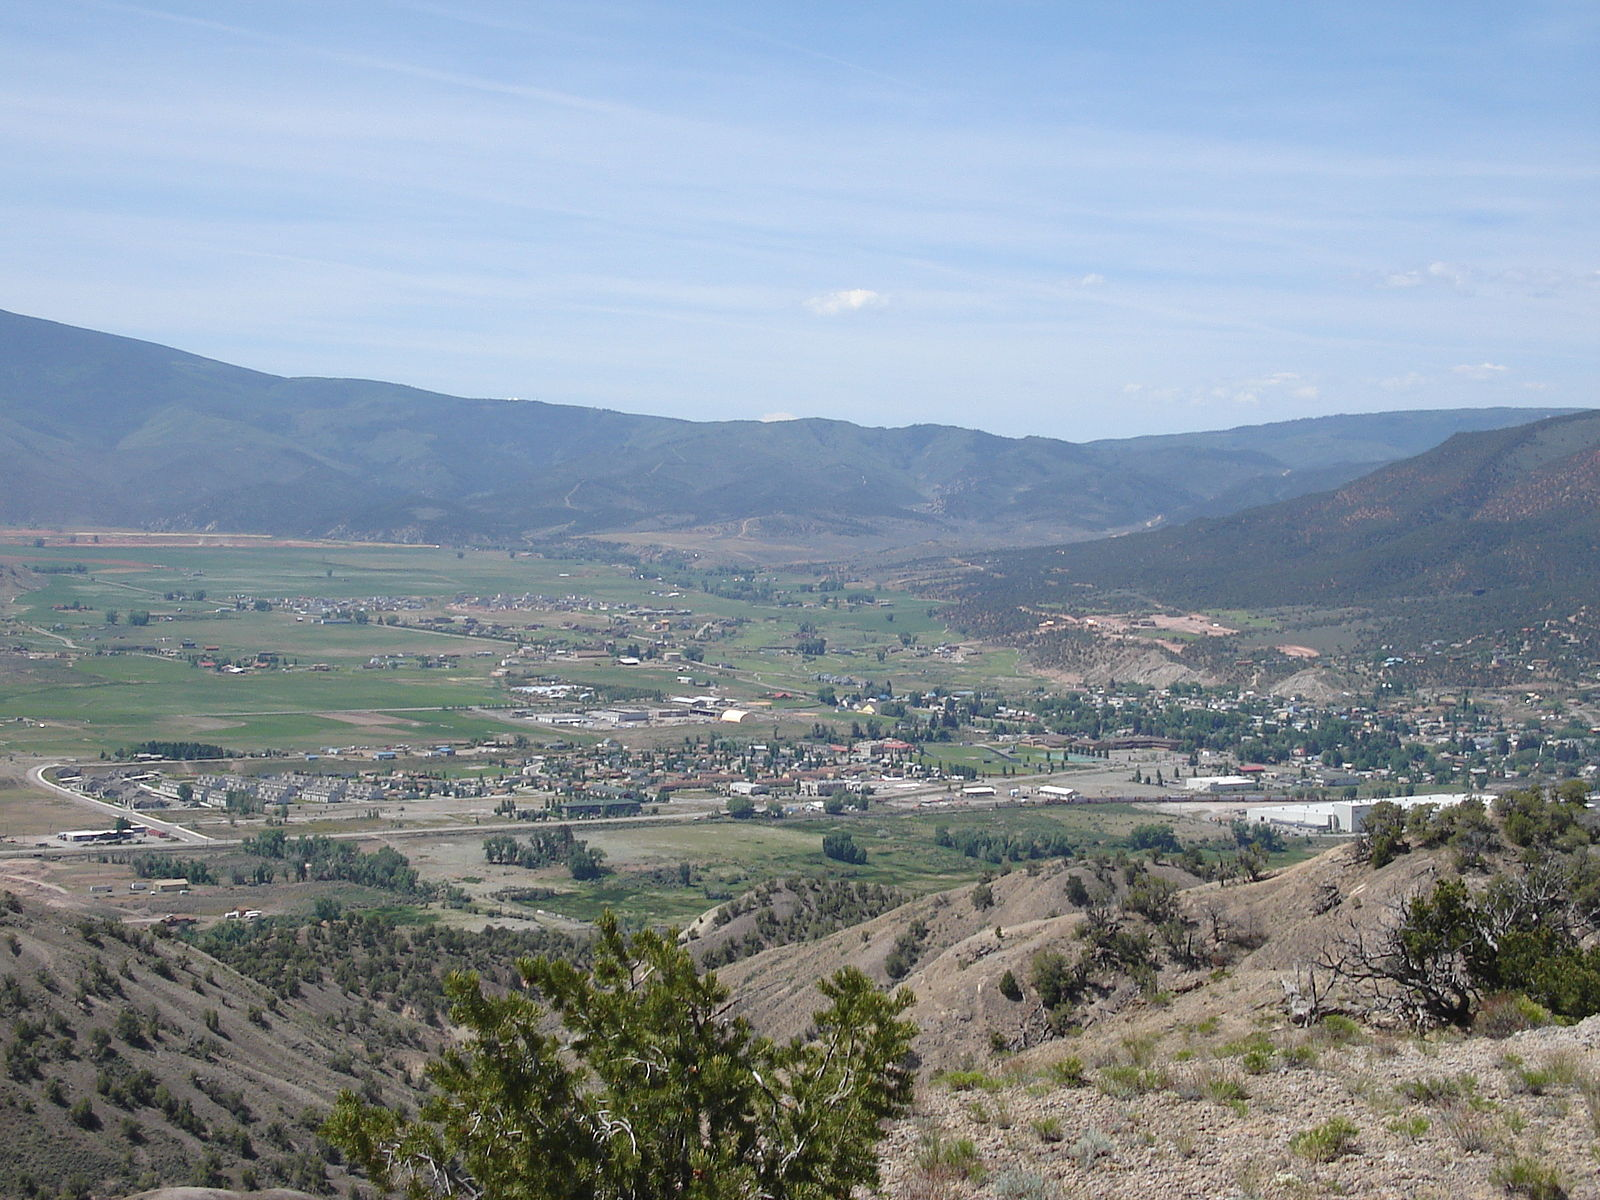
\includegraphics[width=\linewidth]{Images/Gypsum.jpg}
\bigskip
\item[]
\begin{center}
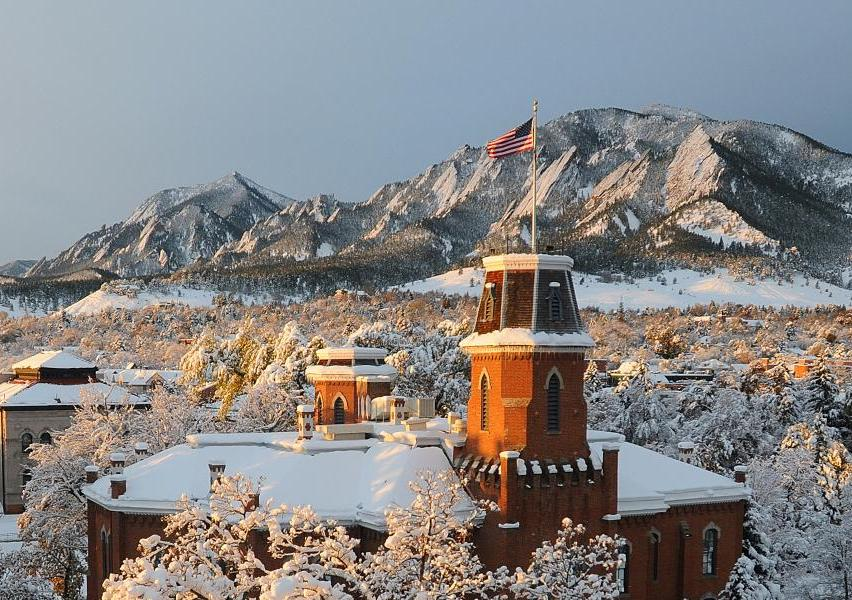
\includegraphics[width=\linewidth]{Images/Boulder.jpg}
\end{center}
\end{itemize}
\end{minipage}
\end{center}
\end{frame}

\begin{frame}\frametitle{Matsen Group}
\begin{minipage}{0.49\linewidth}
\begin{itemize}
\bigskip
\item R.A. for Erick Matsen's group at the Fred Hutch
\bigskip
\item We develop methods to analyze DNA sequences
\bigskip
\item Computational phylogenetics \& immunology
\end{itemize}
\end{minipage}
\begin{minipage}{0.49\linewidth}
\begin{itemize}
\item[]
\begin{center}
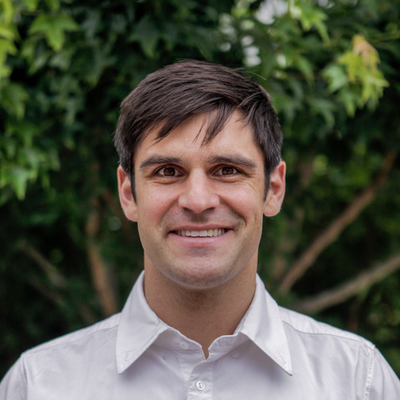
\includegraphics[width=0.7\linewidth]{Images/Erick.png}
\end{center}
\item[]
\begin{center}
\includegraphics[width=0.8\linewidth]{Images/Hutch.jpg}
\end{center}
\end{itemize}
\end{minipage}
\end{frame}

\begin{frame}\frametitle{Research interests}
\begin{minipage}{0.48\linewidth}
\begin{adjustbox}{max totalsize={\textwidth}{.83\textheight},center}
\begin{tikzpicture}
\node[align=center](helix){
\includegraphics[width=\linewidth]{Images/Helix.png}};

\node[below left=5 cm and -2 cm of helix](sequences){
\scalebox{2.5}{
$
\begin{matrix}
\mathtt{GAGGTGCAG...} \\
\mathtt{CAGGTGCAG...} \\
\vdots \\
\mathtt{CATCTATCC...}
\end{matrix}
$
}
};
\node[below right=5 cm and -2 cm of helix](protein){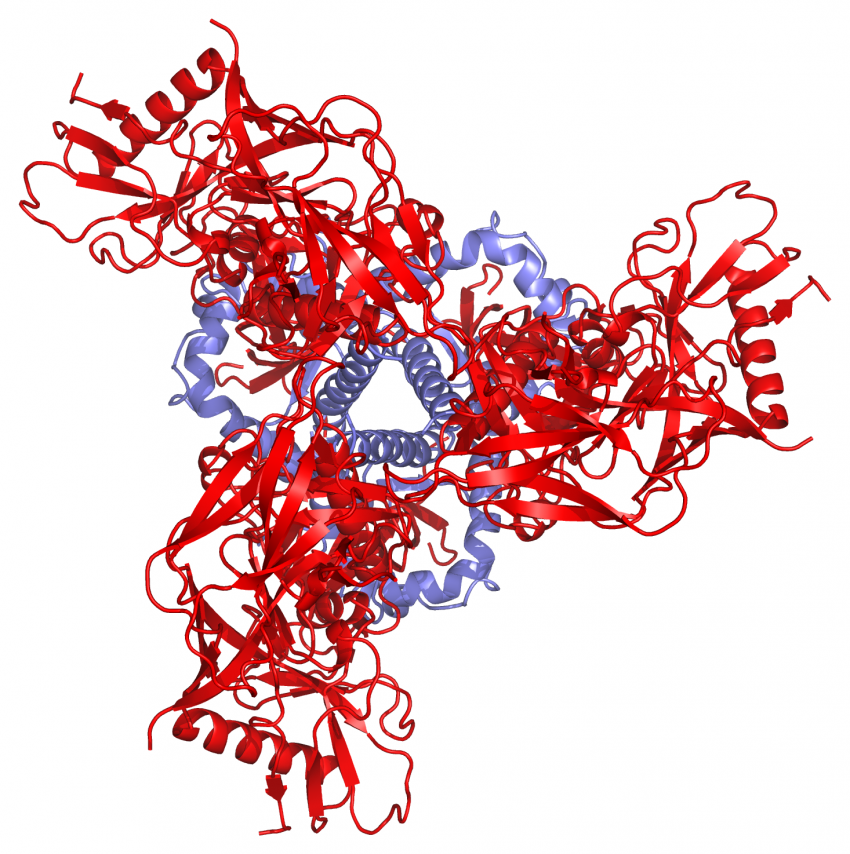
\includegraphics[width=\linewidth]{Images/Protein.png}};

\node[below=0.1 cm of helix](helix_caption){\Huge DNA molecule};
\node[below=0.1 cm of helix_caption](space){};
\node[below=0.1 cm of sequences](seq_caption){\Huge DNA sequences};
\node[below=0.1 cm of protein](protein_caption){\Huge Proteins!};

\draw[->, line width=2pt] (space) -- (sequences);
\draw[->, line width=2pt] (space) -- (protein);

\end{tikzpicture}
\end{adjustbox}
\end{minipage}
\hfill
\begin{minipage}{0.49\linewidth}
\begin{center}
\begin{itemize}
\item
Broad: \emph{computational biology}
\bigskip
\item
More specific: \emph{computational/statistical immunology}
\bigskip
\item
\textbf{More} specific: I analyze DNA sequences of B and T cell receptors (BCRs/TCRs) 
\bigskip
\item
Lots and lots of sequenced DNA data to have fun with!
\end{itemize}
\end{center}
\end{minipage}
\end{frame}

\begin{frame}\frametitle{BCRs and TCRs}
\begin{minipage}{0.49\linewidth}
\begin{itemize}
\item
Proteins that identify and deal with foreign invaders like viruses or bacteria
\bigskip
\item
\emph{Very} critical to the adaptive immune system
\bigskip
\item
Hugely important for vaccine design, understanding cancer/HIV, \& other public health policies
\end{itemize}
\end{minipage}
\begin{minipage}{0.49\linewidth}
\begin{center}
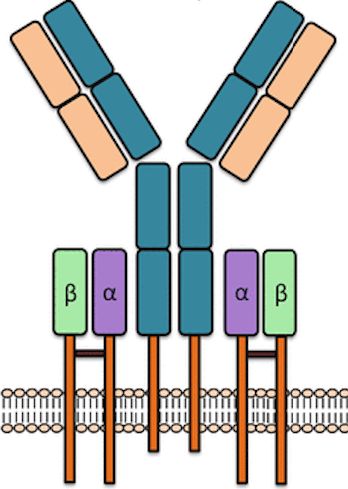
\includegraphics[width=0.4\linewidth]{Images/BCR.png}
\\
\small
B cell receptor
\end{center}
\begin{center}
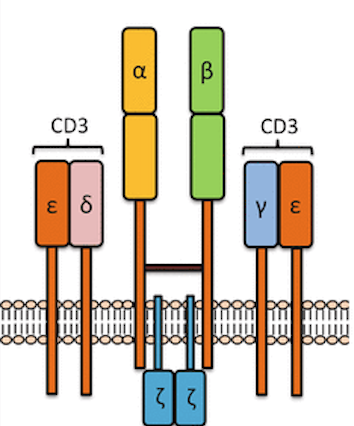
\includegraphics[width=0.4\linewidth]{Images/TCR.png}
\\
\small
T cell receptor
\end{center}
\end{minipage}
\end{frame}

\section{Repertoire summaries and comparisons}

\begin{frame}\frametitle{Motivation}
Immune repertoire sequence datasets are large and complex:
\begin{center}
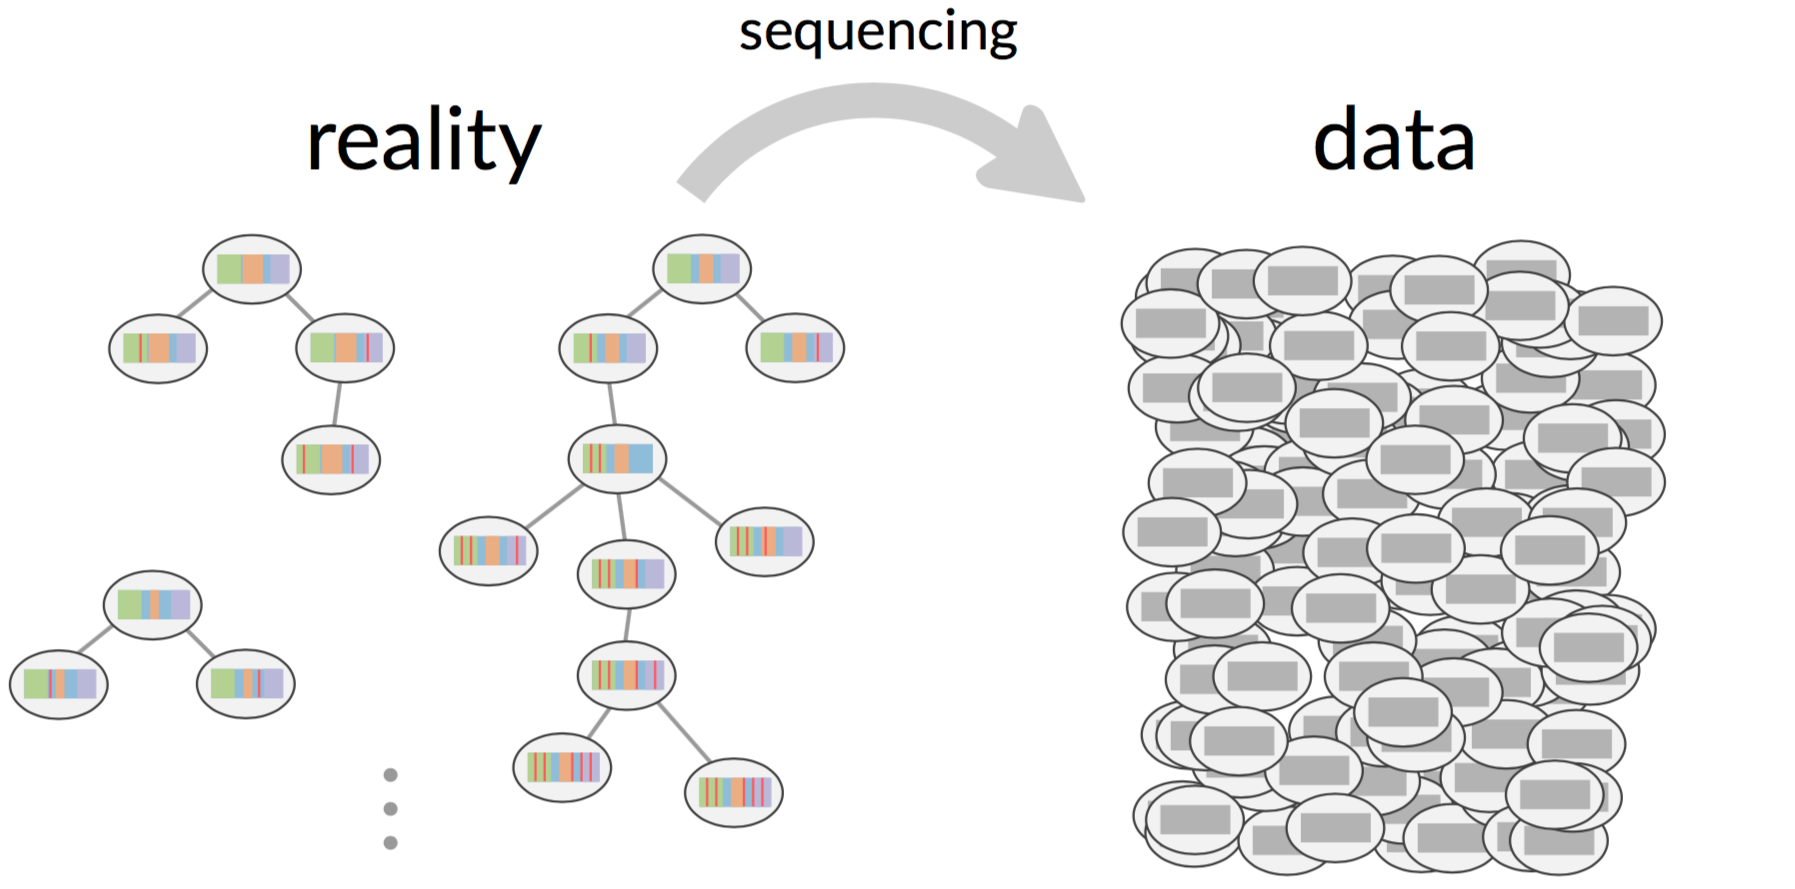
\includegraphics[width=\linewidth]{Images/reality-data.png}
\end{center}
$\implies$ How should we characterize them?
\end{frame}

\begin{frame}\frametitle{Goals}
\begin{itemize}
\item
Idea: Summary statistics reduce a repertoire to numerical \\ (comparable!) quantities
\bigskip
\item
Goal: Build a comprehensive framework for repertoire characterization and comparison via \emph{lots} of summary statistics
\bigskip
\item
Goal: Evaluate the statistics (e.g. robustness to noise, orthogonality) 
\end{itemize}
\end{frame}

\begin{frame}\frametitle{Coming up with summaries}
\begin{itemize}
\item
Teamed up with many scientists in the Adaptive Immune Receptor Repertoire (AIRR) community:
\bigskip
\item[]
\begin{center}
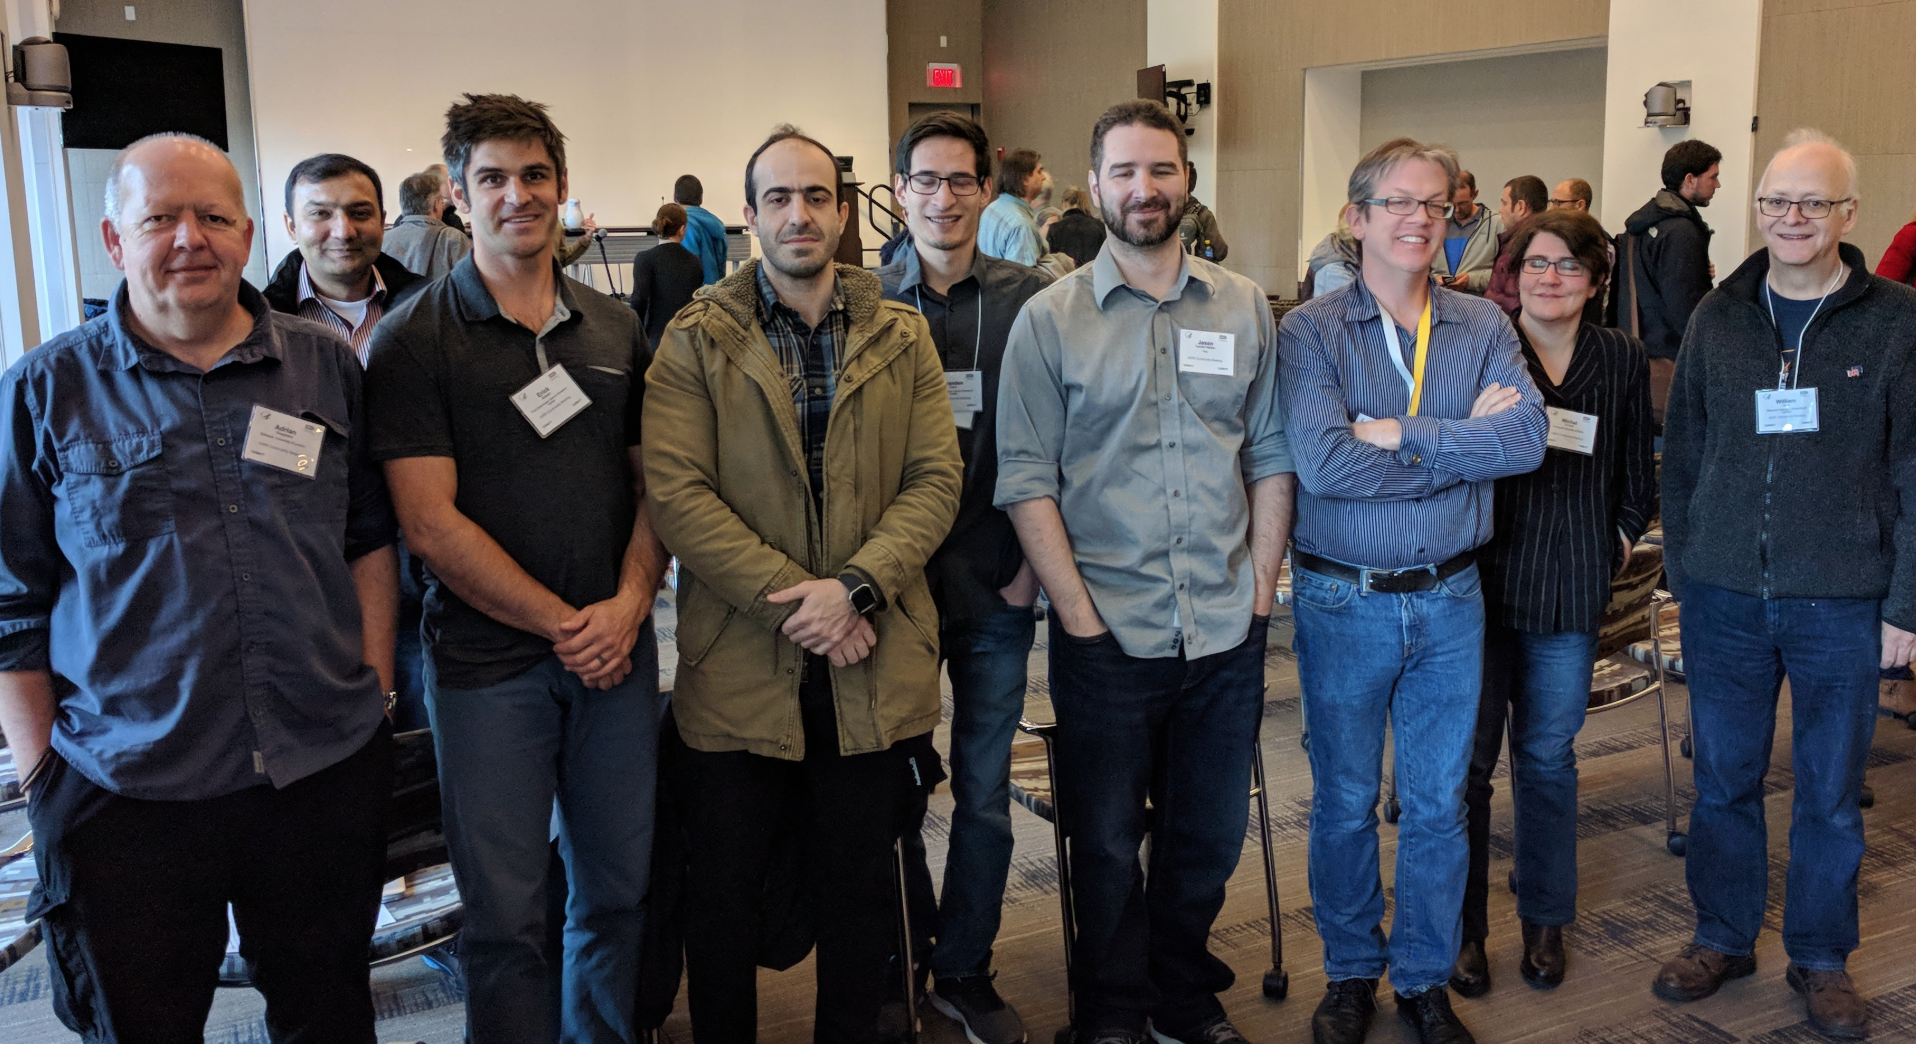
\includegraphics[width=0.9\linewidth]{Images/AIRR.png}
\end{center}
\bigskip
\item
Came up with many stats, from simple DNA stats to specific, complex B/TCR summaries
\end{itemize}
\end{frame}

\begin{frame}\frametitle{Current table of (38) statistics}
\fontsize{5}{7.5}\selectfont
\begin{tabular}{c|c|c|c|c}
    Summary statistic & Annotations & Clustering & Phylogeny & Implementation
\\
\hline \hline
Pairwise distance distribution & No & No & No & \texttt{stringdist} \\
$k$th nearest neighbor distribution & No & No & No & \texttt{stringdist} \\
GC-content distribution & No & No & No & \texttt{ape} \\
Hot/cold spot motif count distribution & No & No & No & \texttt{Biostrings} \\
%BJO Hmm... we never really did much with this (i.e. the Eulerian path paper). Maybe we should discuss?
$k$mer frequency & No & No & No & TBD \\
\hline
Distance from naive to mature distribution & Yes & No & No & \texttt{stringdist} \\
%BJO Another one we kind of skipped over.
$k$th nearest neighbor (V-sequence) distribution & Yes & No & No &\texttt{stringdist},  \texttt{sumrep} \\
CDR3 length distribution & Yes & No & No & Tool-provided \\
Joint distribution of germline gene use & Yes & No & No & \texttt{sumrep} \\
Pairwise CDR3 distance distribution & Yes & No & No & \texttt{stringdist} \\
Hydrophobicity distribution & Yes & No & No & \texttt{Peptides} \\
Atchley factors distribution & Yes & No & No & \texttt{HDMD} \\
Aliphatic index distribution & Yes & No & No & \texttt{Peptides} \\
G.R.A.V.Y. index distribution & Yes & No & No & \texttt{alakazam} \\
Per-gene substitution rate & Yes & No & No & Tool-provided + \texttt{sumrep} \\
Per-gene-per-position substitution rate & Yes & No & No & Tool-provided + \texttt{sumrep} \\
Per-base mutability model & Yes & No & No & \texttt{shazam} \\
Per-base substitution model & Yes & No & No & \texttt{shazam} \\
%BJO This one doesn't depend on fit-star, right?
%EM Yes, but we could just count Ts vs Tv, call it a "ratio" and drop the model-based rigor.
Transition/transversion ratio distribution & Yes & No & No & \texttt{sumrep} \\
Positional distance between mutations distribution & Yes & No & No & \texttt{sumrep}  \\
Distance from naive to mature distribution & Yes & No & No & \texttt{stringdist} \\
V/D/J deletion/insertion lengths distribution & Yes & No & No & Tool-provided \\
Transition matrix for insertions & Yes & No & No & \texttt{sumrep} \\
\hline
Cluster size distribution & Yes & Yes & No & Custom \\
Hill numbers (diversity indices) & Yes & Yes & No & \texttt{alakazam} \\
Selection estimates & Yes & Yes & No & \texttt{shazam} \\
%BJO blocked due to fit-star
Transition/transversion rates & Yes & Yes & No & Tool-provided \\
\hline
Sackin index distribution & Yes & Yes & Yes & \texttt{CollessLike} \\
Colless-like index distribution & Yes & Yes & Yes & \texttt{CollessLike} \\
Cophenetic index distribution & Yes & Yes & Yes & \texttt{CollessLike} \\
%BJO To be delineated
Graph-theoretical features & Yes & Yes & Yes & TBD \\
\end{tabular}
\end{frame}

\begin{frame}\frametitle{Univariate distribution plots}
\begin{center}
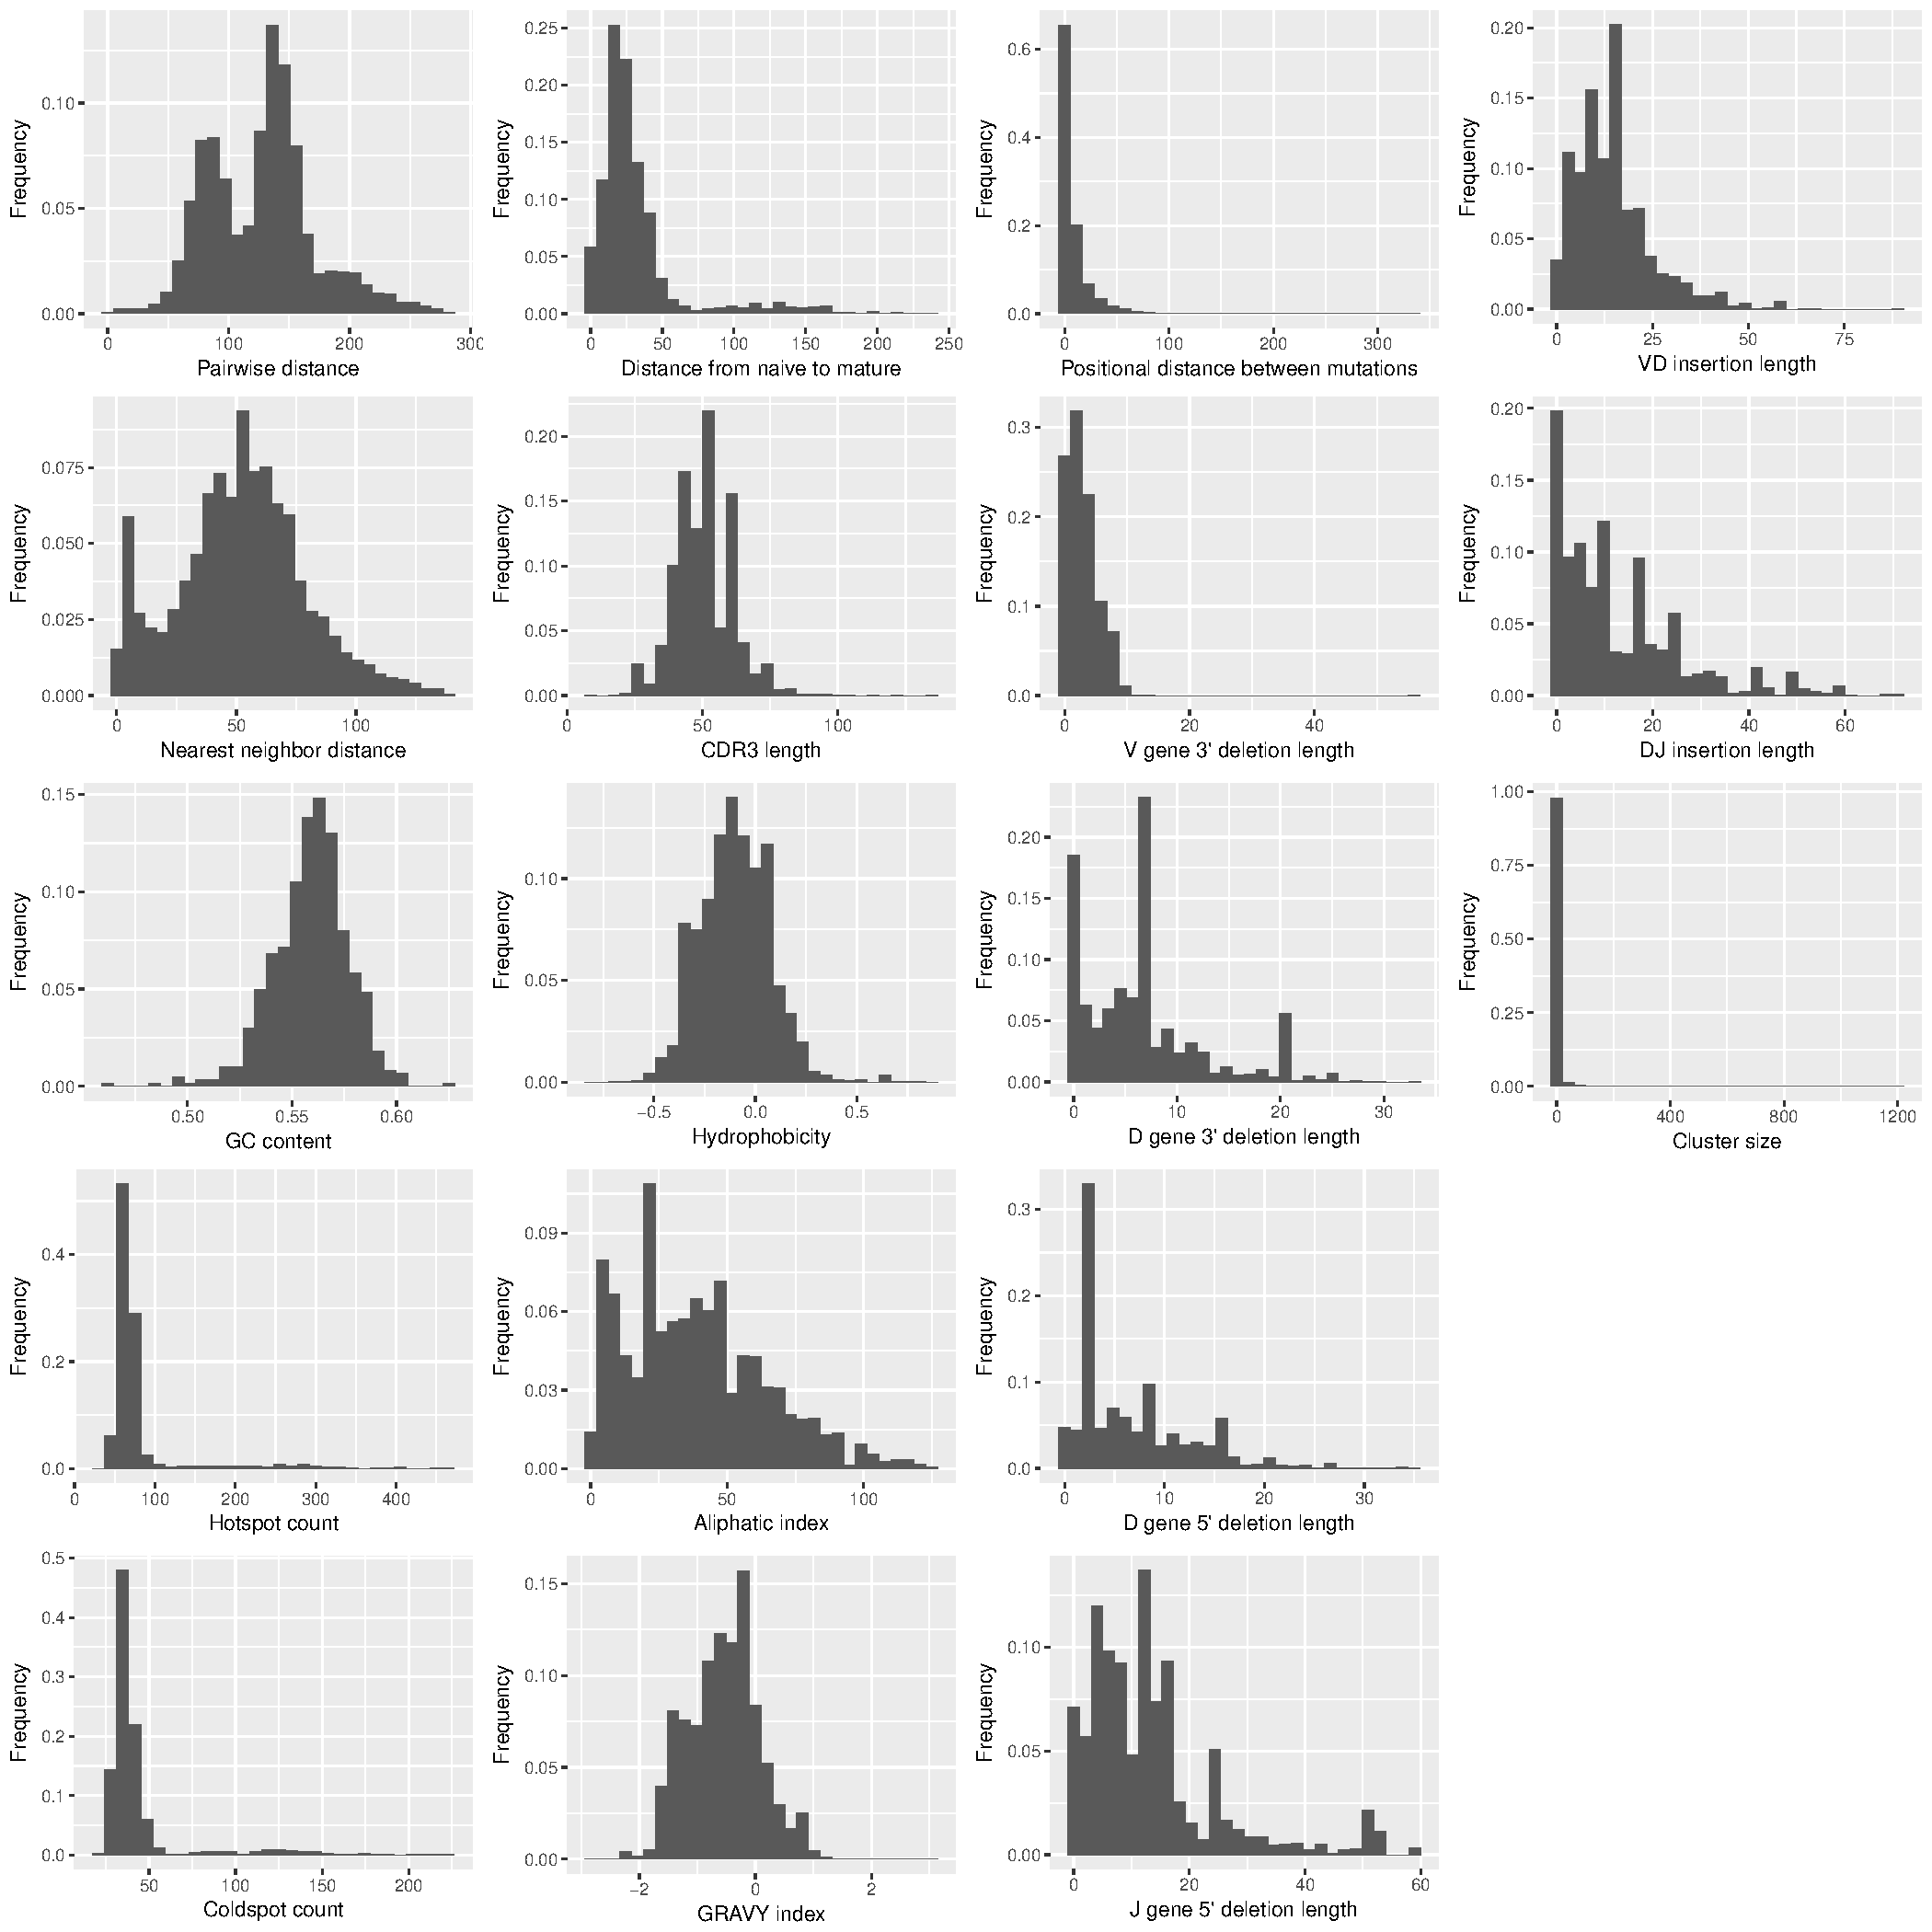
\includegraphics[width=0.75\linewidth]{Images/master_plot.pdf}
\end{center}
\end{frame}

\section{Generative model validation}

\begin{frame}\frametitle{Motivation}
Design and implementation of models is also complex:
\begin{center}
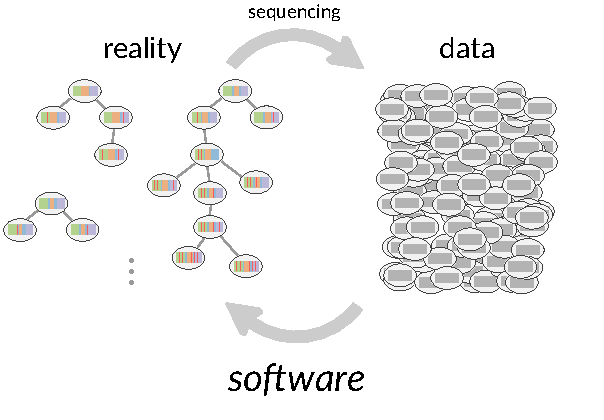
\includegraphics[width=0.8 \linewidth]{Images/bcell-mess-software.pdf}
\end{center}
$\implies$ How should we benchmark them?
\end{frame}

\begin{frame}\frametitle{Motivation}
One (common) way to benchmark: 
\begin{center}
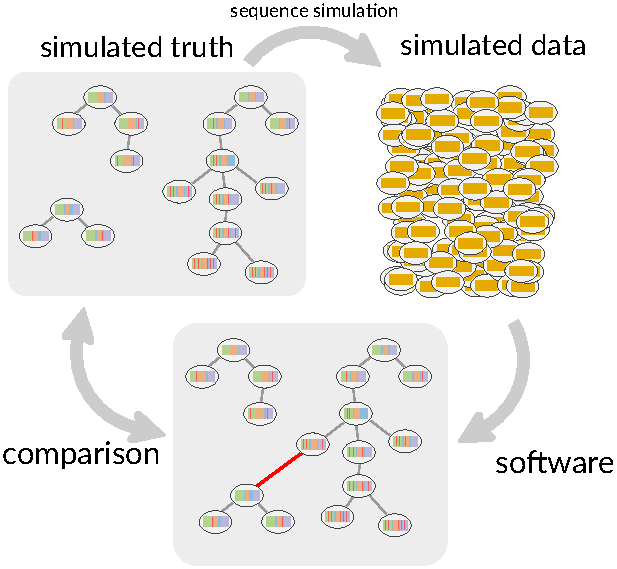
\includegraphics[width=0.7\linewidth]{Images/bcell-mess-simulation.pdf}
\end{center}
\end{frame}

\begin{frame}

\begin{center}\frametitle{Motivating example: Nearest-neighbor distances}
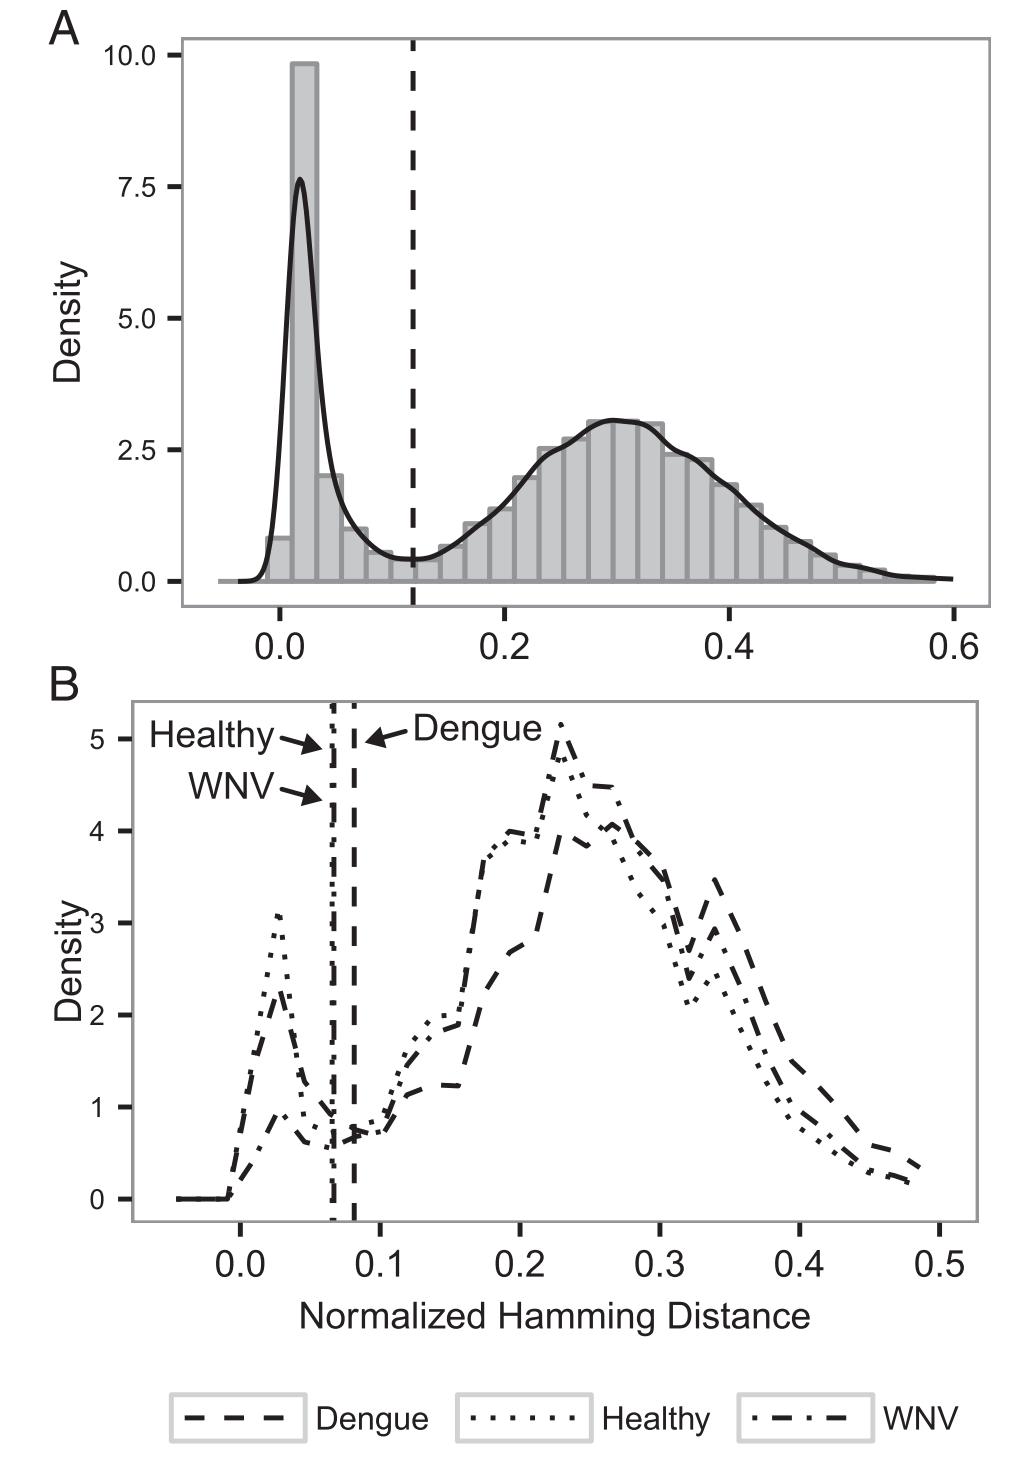
\includegraphics[width=0.4\linewidth]{Images/Dengue.png}
\end{center}
Simulation (top) looks very different than observations (bottom)
\end{frame}

\begin{frame}\frametitle{Goals}
\begin{itemize}
\item
As discussed, we need to benchmark \emph{inferential} tools
\bigskip
\item
This often requires reliable \emph{simulation} tools
\bigskip
\item
Idea: Use our summary statistics framework to assess a simulator's quality
\bigskip
\item
Goal: an automated system that compares simulations to observations and raises flags when things are off

\end{itemize}
\end{frame}

\begin{frame}\frametitle{Prior work}
\begin{itemize}
\item
There have been extensive evaluations of repertoire simulators focused on particular tools/questions	
\medskip
\begin{itemize}
\item
 Duncan's work for \texttt{partis} simulations
 \bigskip
 \item
 Will's work for \texttt{GCtree} simulations
 \bigskip
 \item
 Recent work for summary stats for selection inference
  \end{itemize}
\bigskip
\item
We aim to extend this by:
\medskip
\begin{enumerate}
\item building a tool that does comparisons for \emph{any} simulator 
\bigskip
\item using a broader swath of metrics agreed-upon by the community
\bigskip
\item creating automated reports with comparison metrics for others to assess
\end{enumerate}
\end{itemize}
\end{frame}

\begin{frame}\frametitle{Comparing experimental and simulated data}
\begin{center}
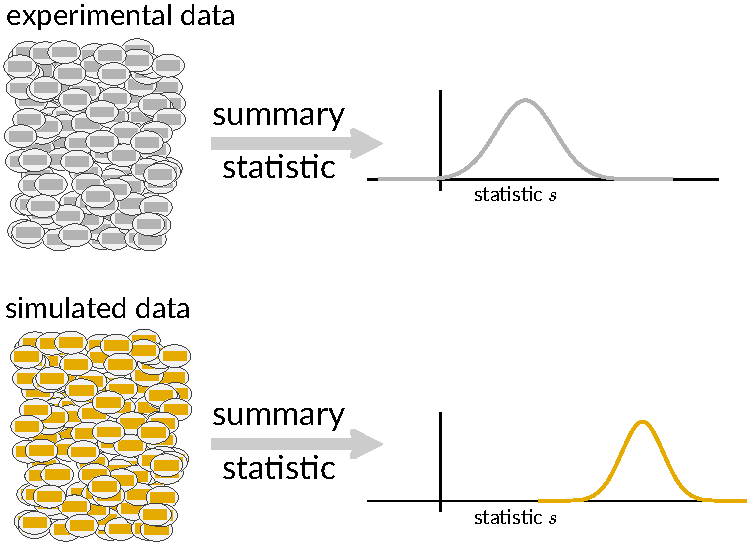
\includegraphics[width=\linewidth]{Images/summary-stats.pdf}
\end{center}
\end{frame}

\begin{frame}\frametitle{Comparing experimental and simulated data}
Good simulators will yield summaries close to those from the observations:
\begin{center}
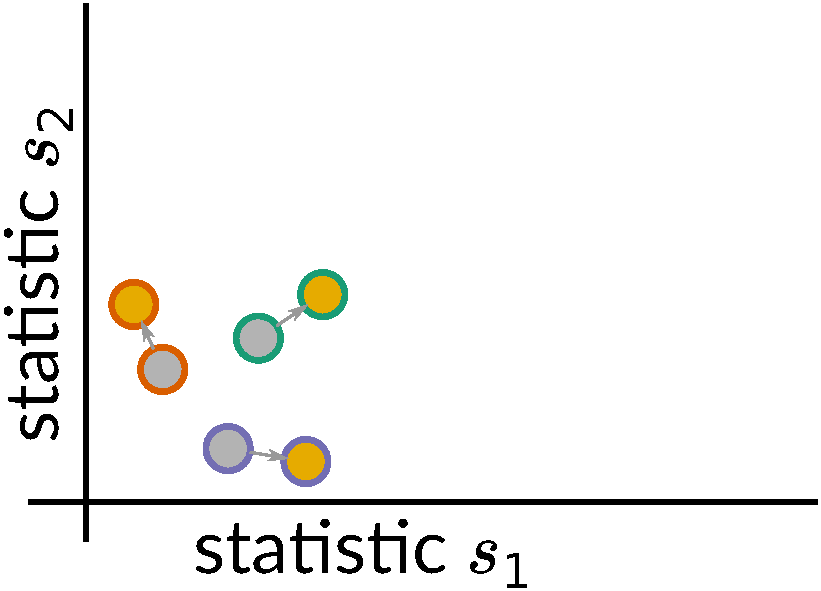
\includegraphics[width=0.65\linewidth]{Images/paired-summary-stats.pdf}
\end{center}
\end{frame}

\begin{frame}\frametitle{Comparing experimental and simulated data}
Worse simulators will yield summaries that are farther from the observations:
\begin{center}
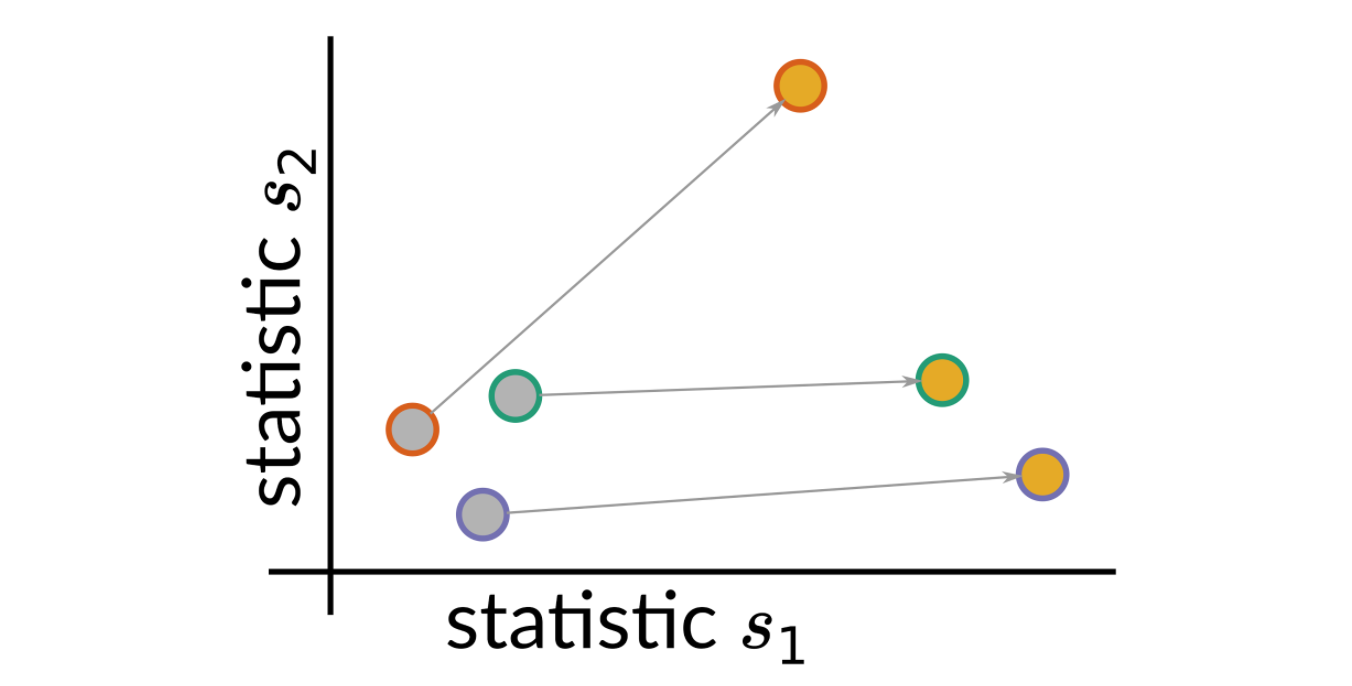
\includegraphics[width=\linewidth]{Images/bad-statistics.png}
\end{center}
\end{frame}

\begin{frame}\frametitle{Comparing summaries using divergences}
\begin{itemize}
\item
We match the divergence method to the nature of $s(\cdot)$
\bigskip
\item
Jenson-Shannon divergence:
\ba
D_{1}(R_1, R_2) =
\text{JS}(R_1 || R_2) = \frac{1}{2} \text{KL}(R_1 || M) + \frac{1}{2} \text{KL}(R_2 || M)
\ea
where $M := \frac{R_1 + R_2}{2}$ and $\text{KL}$ refers to  KL-divergence
\\ \vspace{0.5em} 
Good for \emph{distributions}, e.g. distribution of GC content)
\bigskip
\item
Sum of absolute differences / $\ell_1$-norm
\\ \vspace{0.5em}
Good for vectors/matrices of \emph{count data} (e.g. Hill numbers, VDJ joint gene usage)
\bigskip
\item
Absolute scalar difference \\
(e.g. in-frame percentages)
\end{itemize}
\end{frame}


\begin{frame}\frametitle{Introducing \texttt{sumrep}}
\begin{itemize}
\item
We're building an \texttt{R} package called \texttt{sumrep} (\emph{Sum}mary statistics for BCR/TCR \emph{Rep}ertoires)
\bigskip
\item
Standardized collection of many summary statistics 
\bigskip
\item
Corresponding comparison functions for each summary using a relevant divergence
\bigskip
\item
Mostly on DNA or amino acid sequences, but also clusters, trees, and graphs
\bigskip
\item
Why R? An abundance of many nice libraries, including \texttt{alakazam},
\texttt{ape}, \texttt{Biostrings}, \texttt{Peptides}, \texttt{shazam}, and \texttt{seqinr}
\end{itemize}
\end{frame}

\begin{frame}\frametitle{Summary statistics}
\begin{itemize}
\item
Here, summary statistics $s : \mathcal R \mapsto \mathcal S$ map the set of repertoires $\mathcal R$  to some numerical set $\mathcal S$
\medskip
\item
For example,
\ba
s_\text{GC-content}(R) =
\left(\begin{matrix}
\text{GC-content}(\mathtt{GAGGTGCAG...}) \\
\text{GC-content}(\mathtt{CAGGTGCAG...}) \\
\vdots \\
\text{GC-content}(\mathtt{CATCTATCC...})
\end{matrix} \right) = \begin{pmatrix} 0.481 \\ 0.522 \\ \vdots \\ 0.479  \end{pmatrix}
\ea
\item
$s(R)$ can also be a scalar $\in \reals$ (e.g. in-frame percentage) or $\in \naturals$ (e.g. hot spot counts), vector of arbitrary dimension (e.g. hill numbers), 
or a matrix (e.g. substitution model)
\medskip
\item
Distribution vs single value \\
$\iff$ Vector vs scalar
\\ $\iff$ accuracy vs tractability
\end{itemize}
\end{frame}

\begin{frame}\frametitle{Benchmarking tools}
\begin{itemize}
\item
There are a number of repertoire-simulating tools, including \texttt{partis}, AbSim, IGoR, and IgSimulator
\bigskip
\item
Collection of summaries should provide a thorough picture of the strengths and limitations of different generative models
\bigskip
\item
Indicate where improvements can be made with respect to different summaries of biological/contextual importance
\bigskip
\item
Can add summaries as needed, and omit the ones which seem uninformative
\end{itemize}
\end{frame}

\begin{frame}\frametitle{Numerical study}
\begin{itemize}
\item
Goal: Compare \texttt{partis} annotations and partitions to \texttt{partis} simulations
\bigskip
\item
Annotate three datasets (between 10,000 - 30,000 sequences), and simulate using their inferred parameters
\bigskip
\item
Exploratory: small sample size, and "arbitrary" data
\end{itemize}
\end{frame}


\begin{frame}\frametitle{Numerical study }
\begin{itemize}
\item
Goal: Determine how well each statistic is replicated in the simulations
\bigskip
\item
Scoring formula:
\ba
\text{score}(s) & =
\log \left( \frac{ \frac{1}{|\mathcal I|} \sum_{i \in \mathcal I} \mathcal D \left( R_{i, \text{obs}}, R_{i, \text{sim}} ; s\right) }
    { \frac{1}{\frac{1}{2} |\mathcal I|\left(|\mathcal I| - 1\right)}
        \sum_{\substack{i, j \in \mathcal I \\ i \ne j}} \mathcal D\left(R_{i, \text{obs}}, R_{j, \text{obs}}; s\right) } \right) \\
	& = \log \left( \frac{ \text{average div. of obs. to sim. counterpart} }
					{ \text{average div. of obs. to other obs.} } \right)
\ea 
$R_{i, \text{obs}}$ is the $i$th observed dataset and $R_{i, \text{sim}}$ is the simulation based on the $i$th observed dataset.  
\bigskip
\end{itemize}
\end{frame}

\begin{frame}\frametitle{Scoring results}
\begin{center}
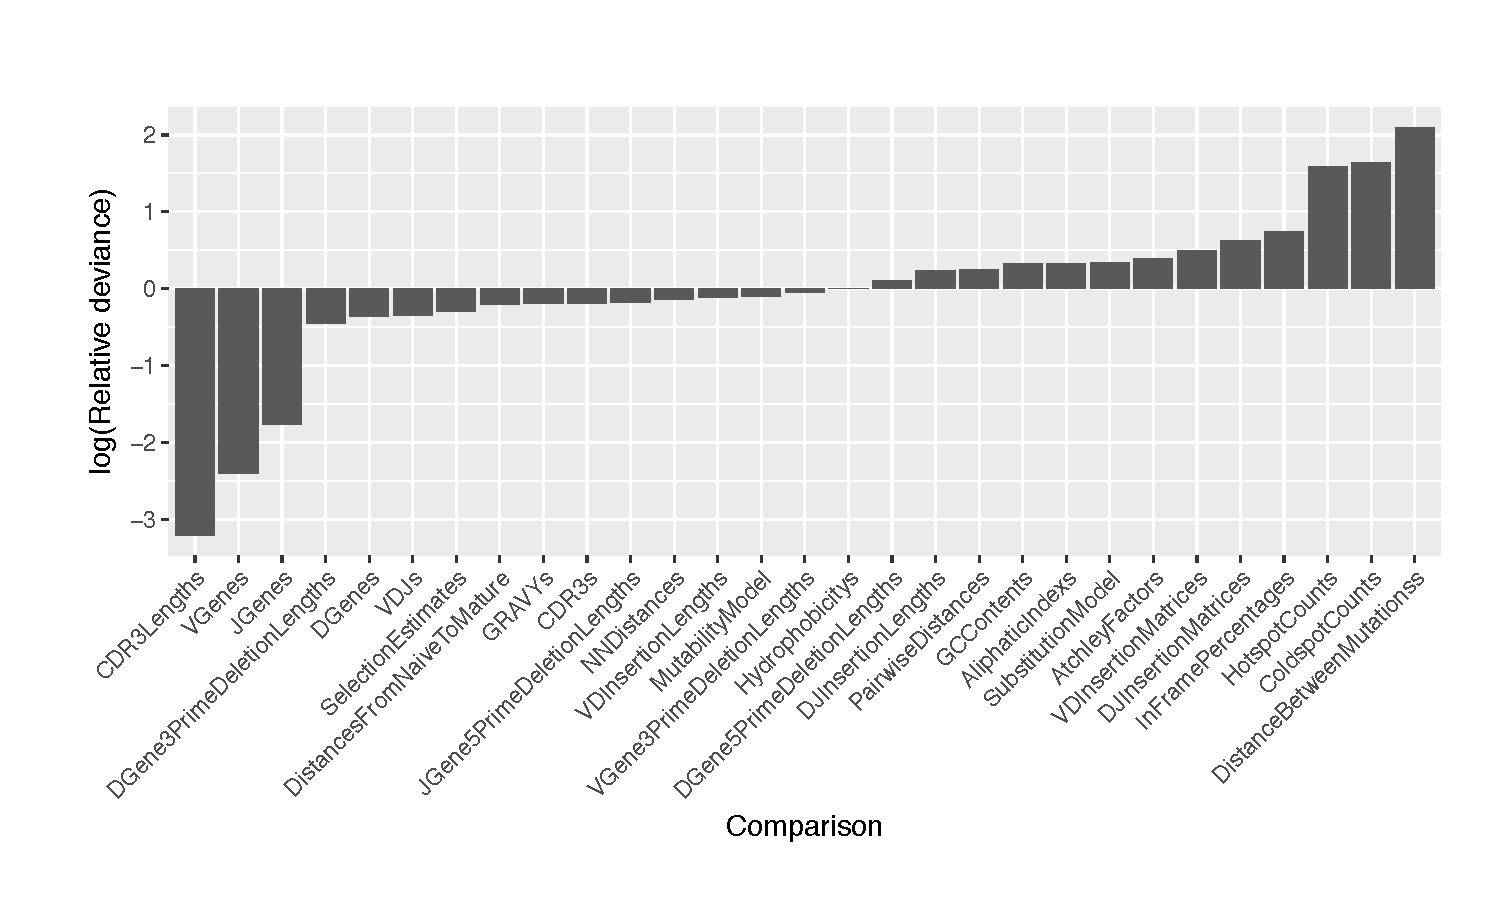
\includegraphics[width=\linewidth]{Images/score_plot.pdf}
\end{center}
\end{frame}

\section{Functional prediction with deep learning}

\begin{frame}\frametitle{Sequences and binding}
\begin{itemize}
\item
Different sequences bind to different invaders
\bigskip
\item
Similar DNA sequences may or may not bind similar invadeers
\item
\bigskip
In fact, very different sequences can bind to the same invader
\bigskip
\item
Can we group sequences by inherent binding similarity?
\end{itemize}
\end{frame}

\begin{frame}\frametitle{Variational autoencoder}
\begin{itemize}
\item
We are using a variational autoencoder (VAE) to infer a relationship between sequences:
\begin{center}
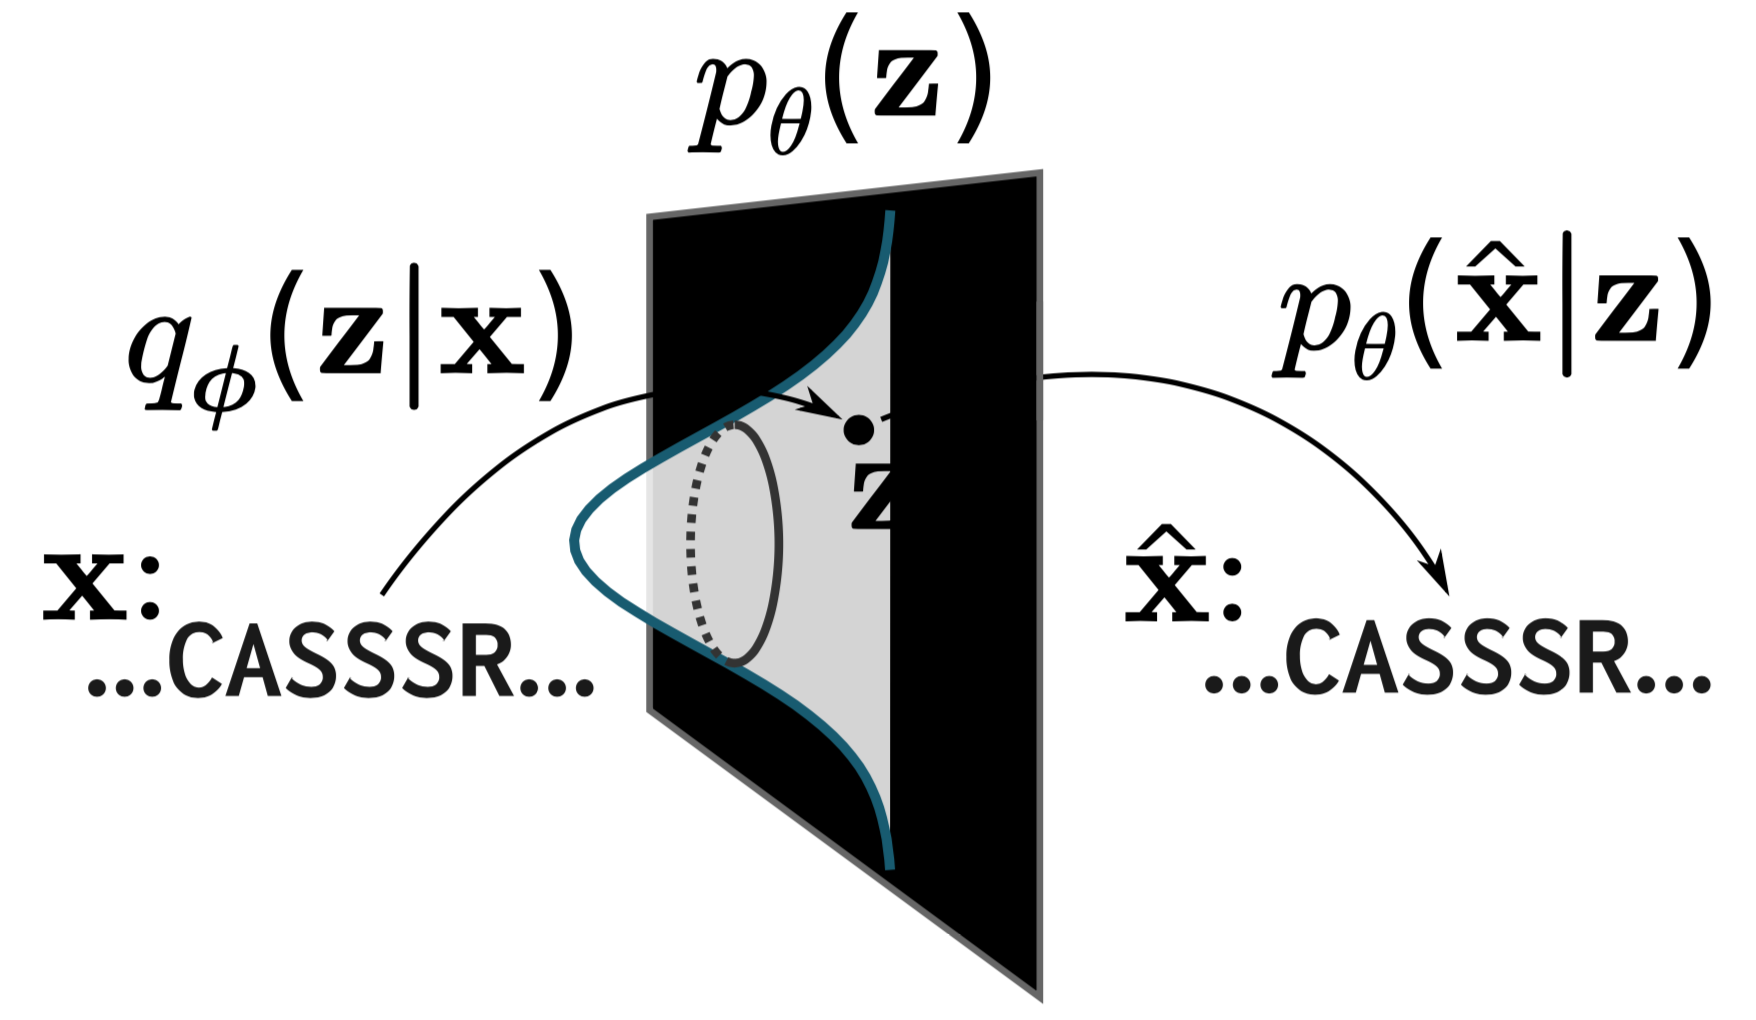
\includegraphics[width=0.7\linewidth]{Images/VAE.png}
\end{center}
\item
Essentially just a deep neural net with an encoder and decoder
\bigskip
\item
You put in a sequence, it gets mapped to a latent space, and then you can generate from this space to get new sequences

\end{itemize}
\end{frame}

\begin{frame}\frametitle{Preliminary results}
\begin{itemize}
\item
Train the VAE on $\approx300,000$ sequences from an individual with cytomegalovirus
\bigskip
\item
Also train IGoR, the current state-of-the-art TCR inference and generative model, on same dataset
\bigskip
\item
Investigate summary distributions for the observed, VAE-simulated, and IGoR-simulated datasets 
\end{itemize}
\end{frame}

\begin{frame}\frametitle{Preliminary results}
\begin{center}
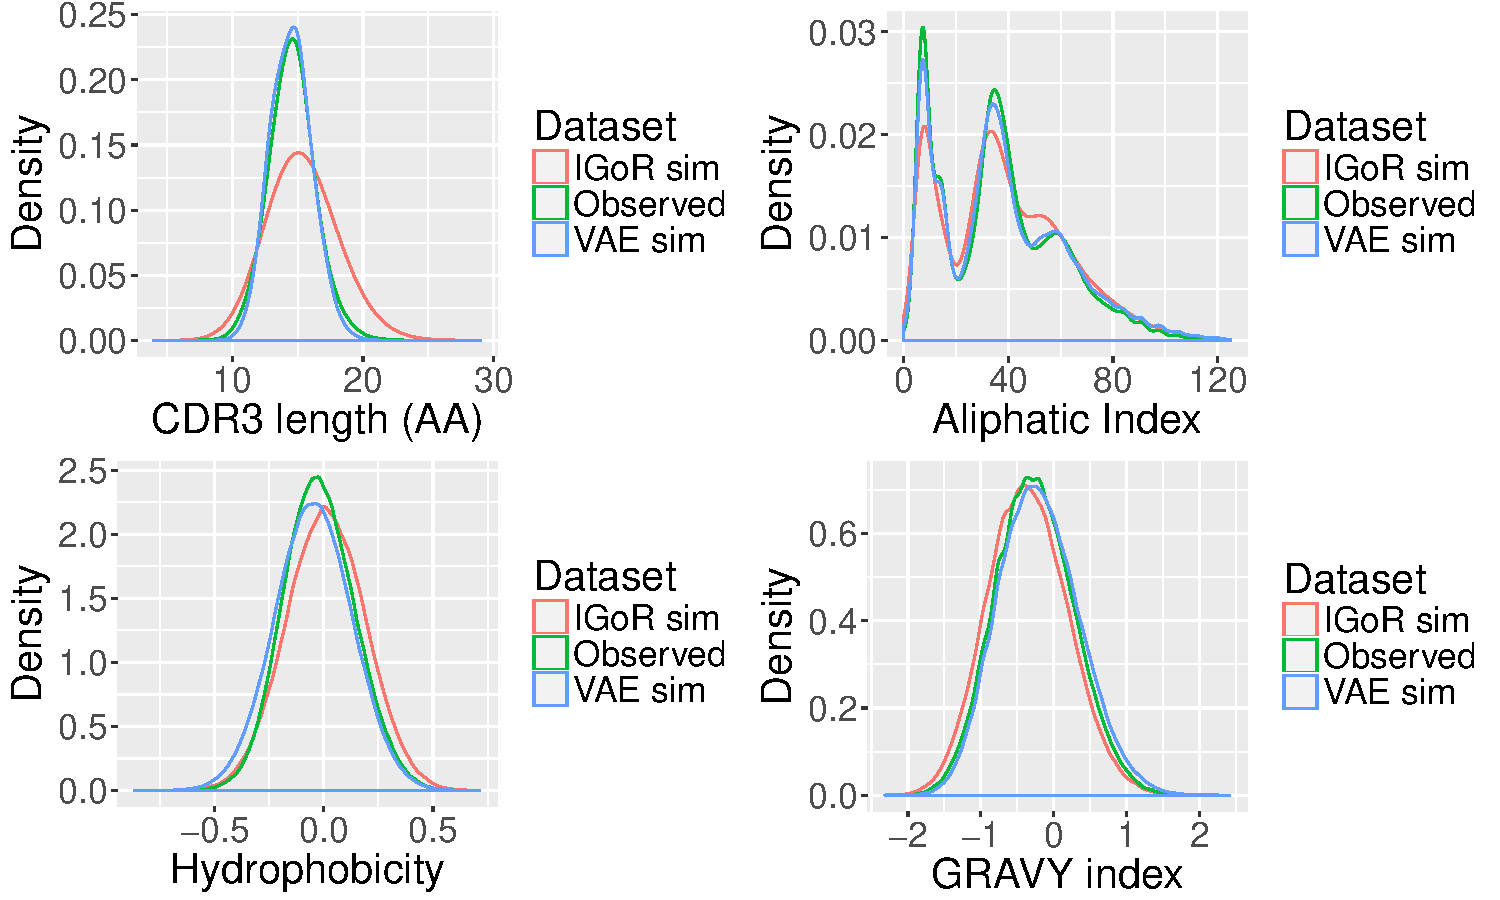
\includegraphics[width=\linewidth]{Images/physiochem.pdf}
\end{center}
\end{frame}

\begin{frame}\frametitle{Preliminary results}
\begin{center}
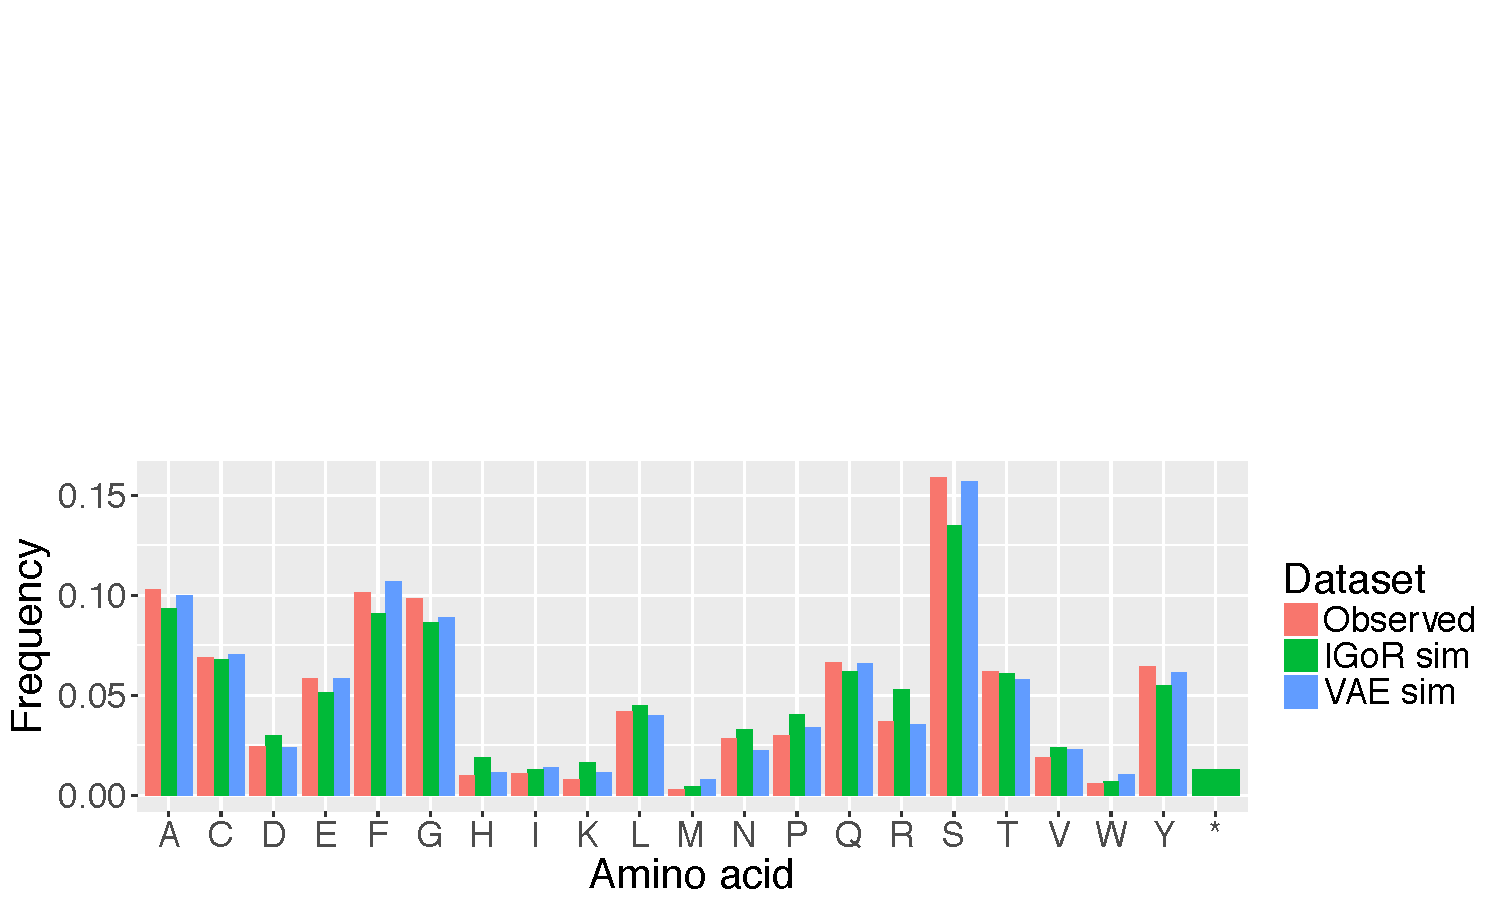
\includegraphics[width=\linewidth]{Images/aa.pdf}
\end{center}
\begin{center}
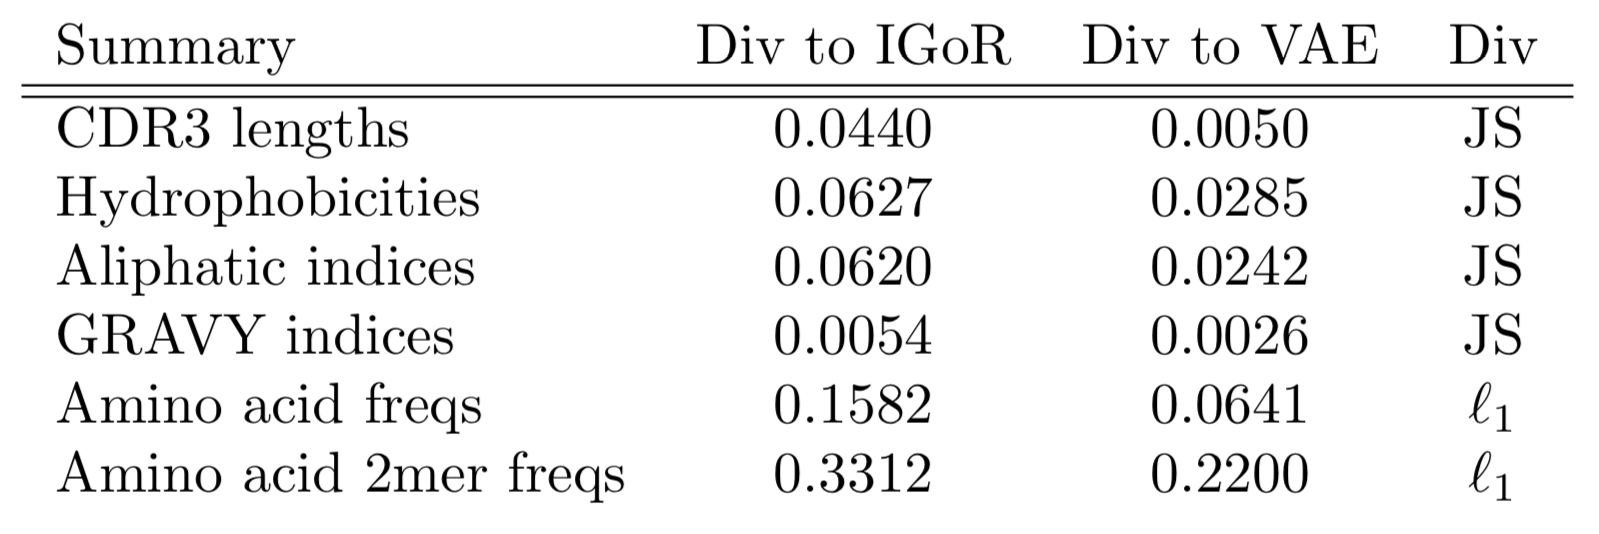
\includegraphics[width=\linewidth]{Images/DivTable.png}
\end{center}
\end{frame}

\begin{frame}\frametitle{Wait... are we just regurgitating sequences?}
\begin{itemize}
\item
We want to make sure we're not overfitting the training data
\bigskip
\item
Idea: use the Birthday Paradox to estimate support of VAE
\end{itemize}
\end{frame}

\section{Conclusion}

\begin{frame}\frametitle{Interested? Start here!}
\begin{center}
\begin{itemize}
\item[]

\includegraphics[width=0.8 \linewidth]{Images/Sompayrac.png}
\bigskip
\item[]
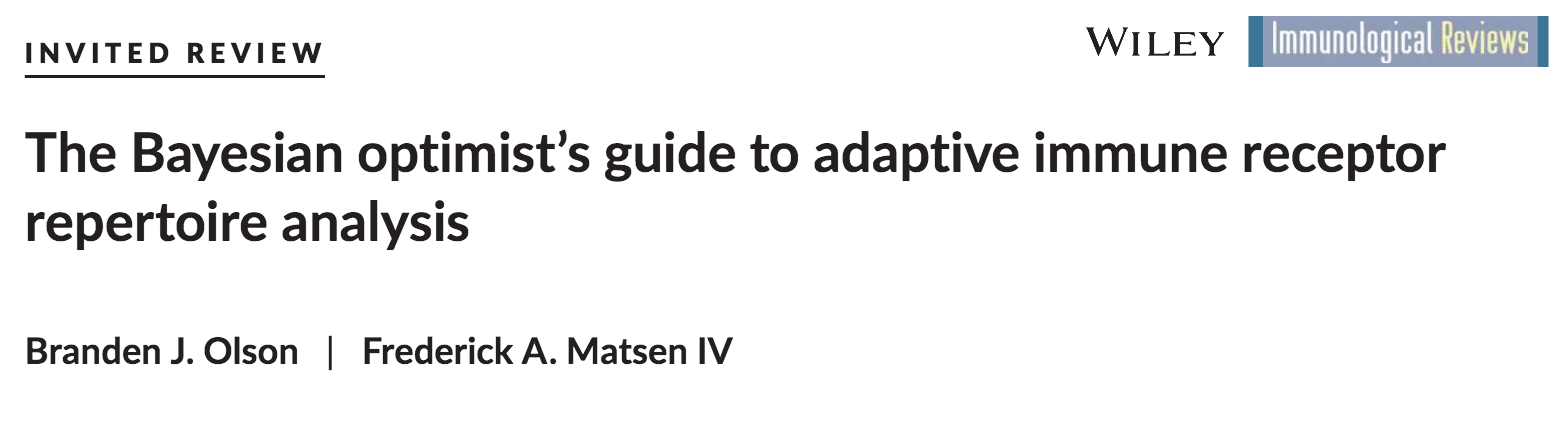
\includegraphics[width=\linewidth]{Images/Optimist.png}
\end{itemize}
\end{center}
\end{frame}

\begin{frame}
\begin{center}
\large
Questions?
\end{center}
\end{frame}


\end{document}























